%!TEX root = ../../terrainbook.tex
% chktex-file 46

\graphicspath{{appendices/ahn/figs/}}

\chapter{LAS \& AHN classification}%
\label{app:ahn}

% TODO: update to AHN4?

The national Dutch AHN3 lidar dataset 
\marginnote{\emph{Actueel Hoogtebestand Nederland} (AHN)}
\marginnote{\url{https://www.ahn.nl}}
is disseminated in the LAZ format (a compressed LAS, see below) and uses the LAS classification codes. 
Figure~\ref{fig:ahn3} shows all the codes that are used in  AHN3. 
\begin{figure*}
  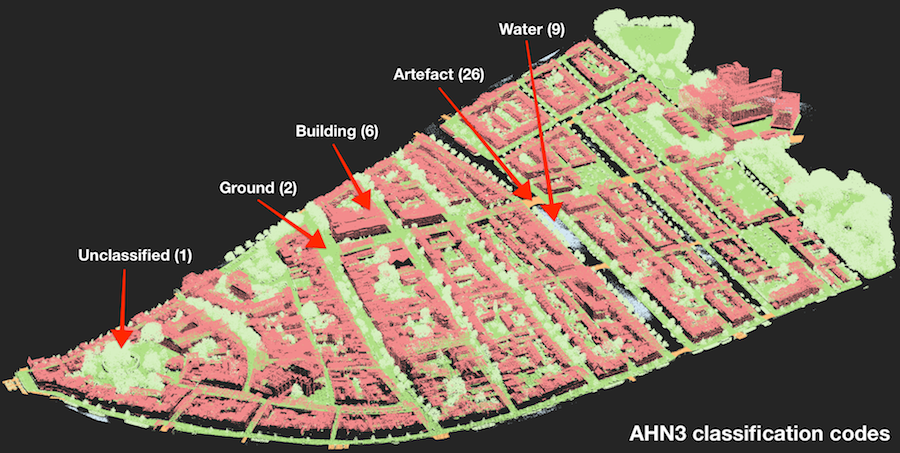
\includegraphics[width=\linewidth]{ahn3.png}
  \caption{Classification codes used in the AHN3 dataset.}%
\label{fig:ahn3}
\end{figure*}
Notice that apart from the pre-defined codes from Table~\ref{tab:las-classes}, it also uses the custom code $26$ for an `artefact' (Dutch: \emph{kunstwerk}) class that includes special infrastructures such as bridges and viaducts. 

Notice that in AHN3 the points representing vegetation are not classified as such, and vegetation is never explicitly classified.
\marginnote{vegetation is classified as $1$/unclassified in AHN3}
The is because the aim of the AHN project is mostly to model dikes and to protect us from floods, and vegetation is not very important for this use-case.
The class $1$ is thus used for vegetation, but other objects such as street furniture (\eg\ lampposts) or cars are also classified as $1$.


% TODO: The standard technically allows for additional user-defined attributes, AHN4 does that actually